\documentclass{article}

\usepackage{graphicx}
\usepackage{tikz}
\usepackage{tikzsymbols}
\usetikzlibrary{calc,patterns,shapes.geometric}
\pagestyle{empty}
\usepackage[margin=0pt]{geometry}
\geometry{papersize={14in,12in}}

\def\centerarc[#1](#2)(#3:#4:#5){\draw[#1] ($(#2)+({#5*cos(#3)},{#5*sin(#3)})$) arc (#3:#4:#5);}

\begin{document}
	\begin{figure}
		\centering
		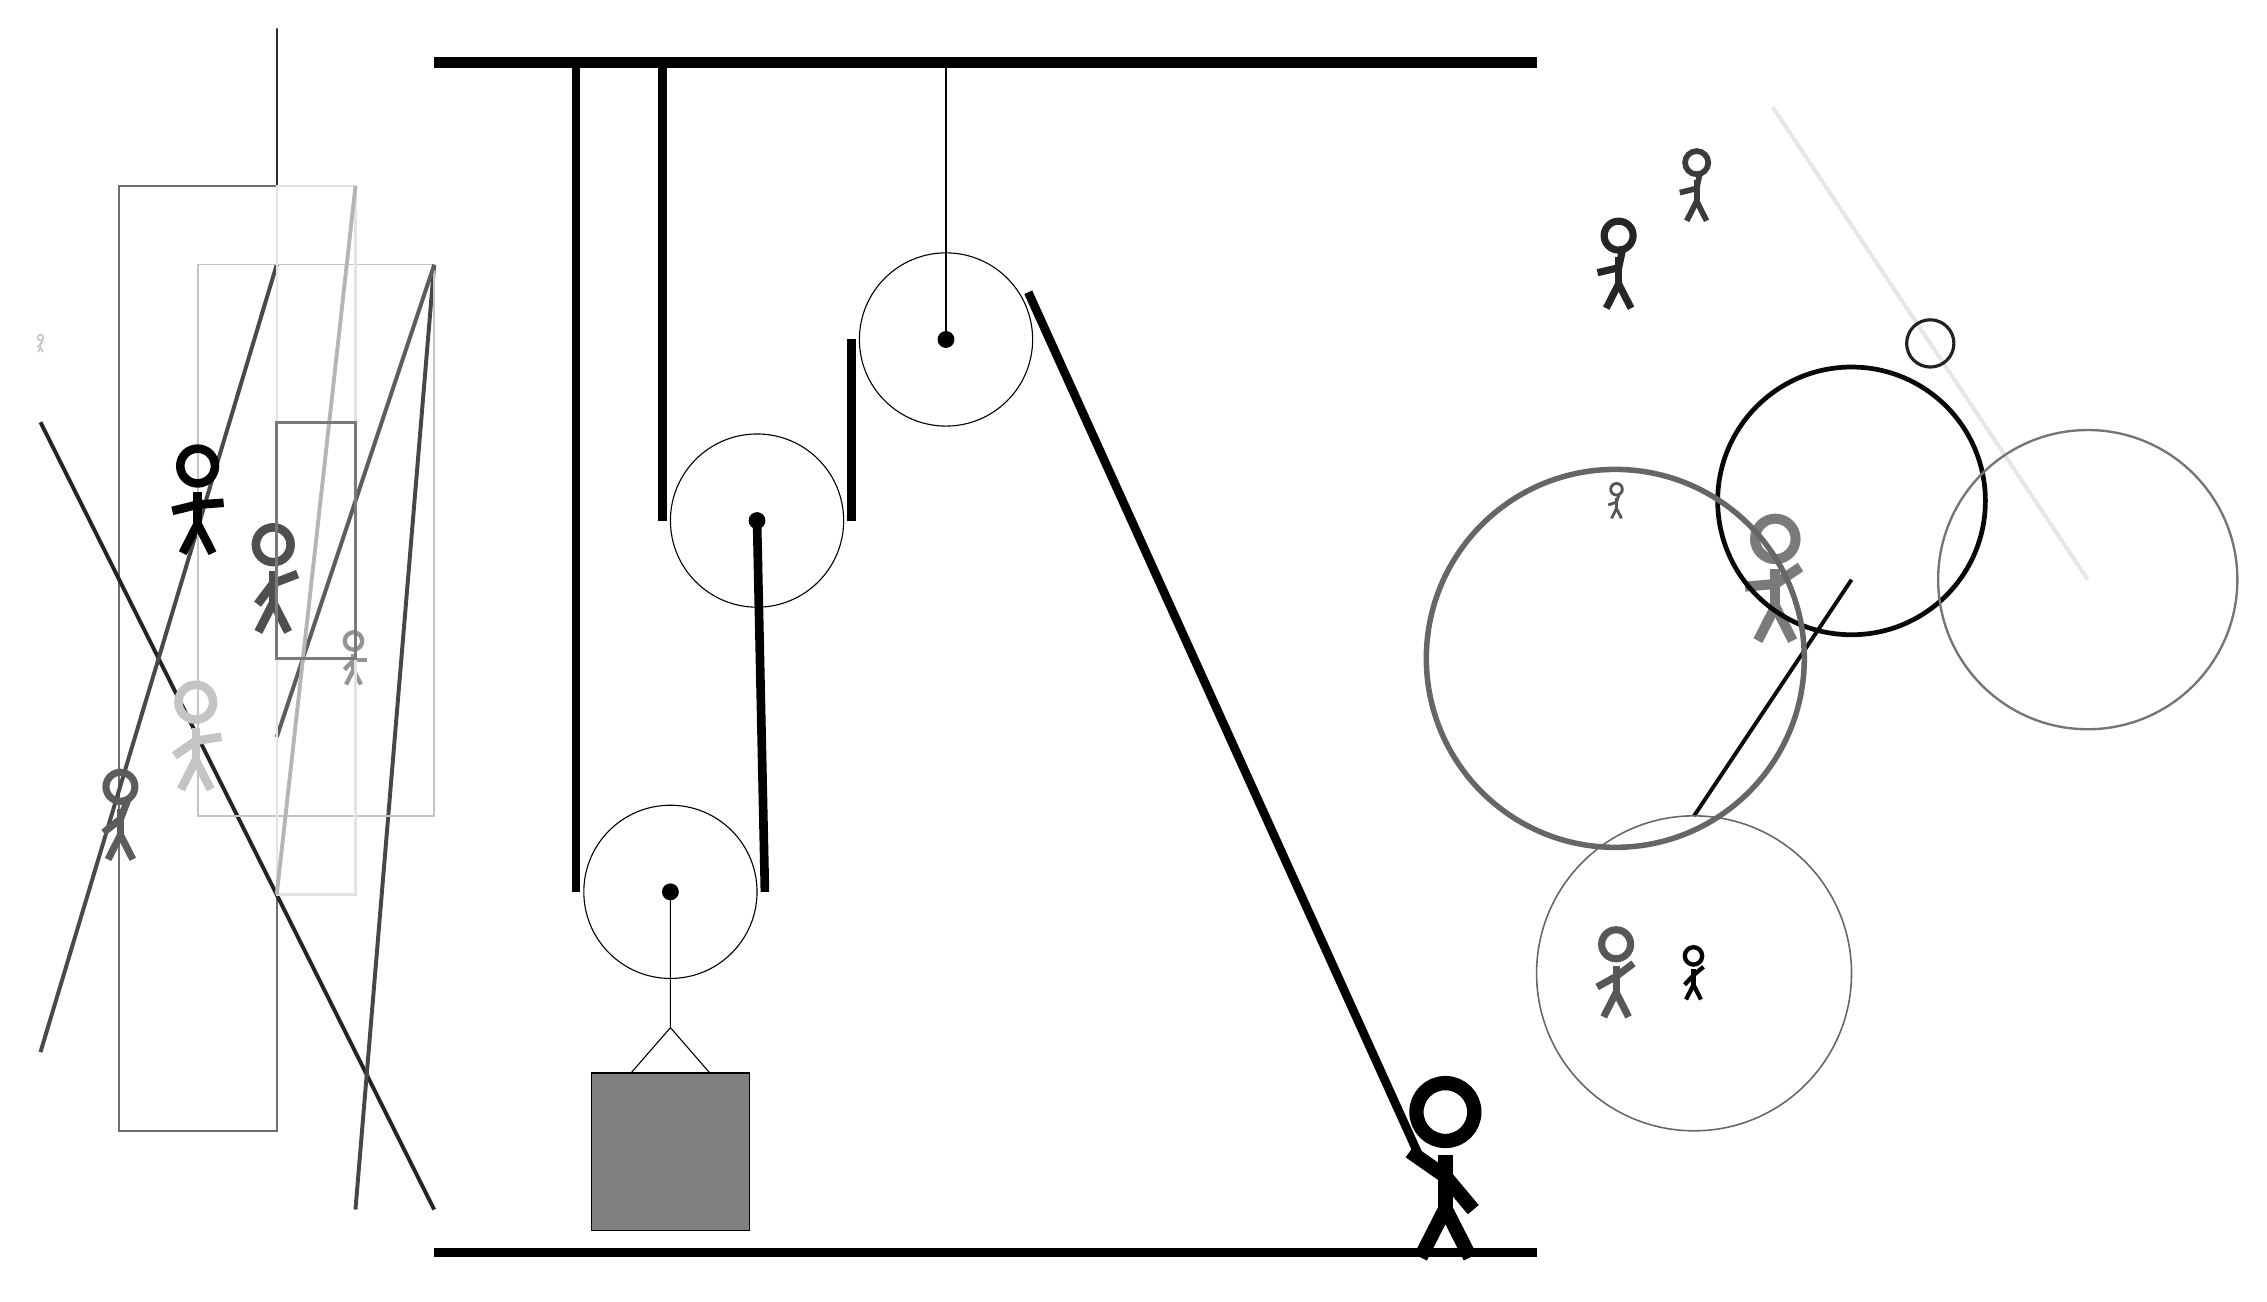
\begin{tikzpicture}
			%%%%% START %%%%%
			
			\draw[fill=black] (-2, 11.5) rectangle (12, 11.625);
			
			\draw (1, 1.035) circle (1.1);
			\draw[fill=black] (1, 1.035) circle (0.1);
			
			\draw (2.1, 5.75) circle (1.1);
			\draw[fill=black] (2.1, 5.75) circle (0.1);
			
			\draw (4.5, 8.05) circle (1.1);
			\draw[fill=black] (4.5, 8.05) circle (0.1);
			\draw[thick] (4.5, 8.05) -- (4.5, 11.5);
			
			\draw (1, 1.035) -- (1, -0.69) -- (0.5, -1.265) -- (1.5, -1.265) -- (1, -0.69);
			\draw[fill=black!50] (0, -1.265) rectangle (2, -3.265);
			
			\draw[line width=1.1mm] (-0.2, 11.5) -- (-0.2, 1.035);
			\centerarc[line width=1.1mm](1, 1.035)(180:360:1.2000000000000002);
			\draw[line width=1.1mm](2.2, 1.035) -- (2.1, 5.75);
			\draw[line width=1.1mm] (0.9, 11.5) -- (0.9, 5.75);
			\centerarc[line width=1.1mm](2.1, 5.75)(180:360:1.2000000000000002);
			\draw[line width=1.1mm](3.3, 5.75) -- (3.3, 8.05);
			\centerarc[line width=1.1mm](4.5, 8.05)(30:180:1.2000000000000002);
			\draw[line width=1.1mm] (5.544, 8.65) -- (10.5, -2.3);
			
			\draw[line width=0.3mm, color=black!73] (-4, 2) rectangle (-4, -2);
			
			\draw [line width=0.4mm, color=black!57](-4, 2) circle (0.0);
			\node[line width=0.7mm, color=black!42] at (-3, 4) {\Strichmaxerl[3][46][0]};
			\draw[line width=0.3mm, color=black!57] (-4, -2) rectangle (-6, 10);
			\draw[line width=0.5mm, color=black!86](-7, 7) -- (-2, -3);
			
			\draw[line width=0.5mm, color=black!95](16, 5) -- (14, 2);
			\draw[line width=0.2mm, color=black!84] (-4, 5) rectangle (-4, 12);
			\draw[line width=0.5mm, color=black!71](-4, 9) -- (-7, -1);
			\node[line width=0.7mm, color=black!69] at (-4, 5) {\Strichmaxerl[6][53][21]};
			\node[line width=0.4mm, color=black!25] at (-7, 8) {\Strichmaxerl[1][51][52]};
			\draw[line width=0.5mm, color=black!10](15, 11) -- (19, 5);
			
			\node[line width=0.6mm, color=black!52] at (15, 5) {\Strichmaxerl[7][5][34]};
			\node[line width=0.4mm, color=black!85] at (13, 9) {\Strichmaxerl[5][13][78]};
			
			\draw[line width=0.5mm, color=black!72](-2, 9) -- (-3, -3);
			\draw [line width=0.6mm, color=black!97](16, 6) circle (1.7);
			\draw[line width=0.2mm, color=black!23] (-2, 2) rectangle (-5, 9);
			\draw[line width=0.5mm, color=black!64](-2, 9) -- (-4, 3);
			
			\node[line width=0.4mm, color=black!64] at (-6, 2) {\Strichmaxerl[5][39][69]};
			\node[line width=0.5mm, color=black!67] at (13, 6) {\Strichmaxerl[2][19][72]};
			\node[line width=0.7mm, color=black!77] at (14, 10) {\Strichmaxerl[4][14][78]};
			\draw [line width=0.4mm, color=black!87](17, 8) circle (0.3);
			\draw [line width=0.7mm, color=black!60](13, 4) circle (2.4);
			
			\draw[line width=0.3mm, color=black!11] (-3, 1) rectangle (-4, 10);
			\draw[line width=0.5mm, color=black!29](-3, 10) -- (-4, 1);
			\draw [line width=0.2mm, color=black!60](14, 0) circle (2.0);
			
			\node[line width=0.5mm, color=black!23] at (-5, 3) {\Strichmaxerl[6][35][9]};
			
			\draw [line width=0.3mm, color=black!54](19, 5) circle (1.9);
			\node[line width=0.2mm, color=black!66] at (13, 0) {\Strichmaxerl[5][29][37]};
			
			\draw[line width=0.4mm, color=black!52] (-4, 4) rectangle (-3, 7);
			
			\node[line width=0.7mm, color=black!100] at (14, 0) {\Strichmaxerl[3][47][40]};
			\node[line width=0.3mm, color=black!99] at (-5, 6) {\Strichmaxerl[6][14][4]};
			
			
			\node at (10.8, -2.5) {\Strichmaxerl[10][-35][-50]};
			
			\draw[fill=black] (-2, -3.5) rectangle (12, -3.6);
			
			%%%%% END %%%%%
		\end{tikzpicture}
	\end{figure}	
\end{document}